\documentclass[11pt]{beamer}
\usetheme{Madrid}
\usepackage[utf8]{inputenc}
\usepackage[spanish]{babel}
\usepackage{amsmath}
\usepackage{amsfonts}
\usepackage{amssymb}
\usepackage{graphicx}
\title{Presentación Moogle}
%\setbeamercovered{transparent} 
%\setbeamertemplate{navigation symbols}{} 
%\logo{} 
%\institute{} 
%\date{} 
%\subject{} 
%\begin{frame}
%\tableofcontents
%\end{frame}
\begin{document}

\begin{frame}
\titlepage

\end{frame}

\begin{frame}{•}
MOOGLE es una aplicación web que permite realizar una búsqueda en archivos TXT de una o 
varias palabras. Como resultado de la búsqueda, se listan los nombres de los ficheros que 
contengan al menos una palabra de la frase.\\

Los ficheros se listan en orden descendente, mostrando al inicio los que contengan mayor 
ocurrencia de la(s) palabra(s) a buscar.
\end{frame}

\begin{frame}
La carpeta donde se encuentra la solución de la aplicación tiene una subcarpeta denominada: 
Content , y es en ella donde deben estar ubicados los archivos TXT.\\

El usuario, al teclear la(s) palabra(s) a buscar, que le hemos estado llamando: query, los procesos 
que se ejecutan son:\\

\begin{itemize}
 \item Limpiar la query: los caracteres de la query se convierten a minúsculas; se eliminan los 
caracteres especiales y estructuras del idioma como: las conjunciones, preposiciones, 
artículos; se eliminan los espacios al inicio y fin de la query, se manejan los acentos.\\

\item Recorrer la lista de palabras de la query y almacenar cada palabra en el diccionario 
dicWordsOfQuery
\end{itemize}
\end{frame}

\begin{frame}
\begin{itemize}
\item Recorrer la lista de archivos TXT que se encuentran en la carpeta Content y almacenar
cada nombre del archivo TXT en el diccionario dicFilesTxt\\

\item Determinar la ocurrencia (cantidad de veces) que se encuentra cada palabra de la query
en cada archivo TXT. Estas cantidades se almacenan en la matriz mtzGeneral.\\

\item Calcular para cada palabra de la query, el valor de TF y almacenarlo en el arreglo 
arrayQueryTF\\

\item Calcular para cada palabra de la query, el valor de IDF y almacenarlo en el arreglo 
arrayQueryIDF\\
\end{itemize}
\end{frame}

\begin{frame}
\begin{itemize}
\item Tomando en cuenta los valores calculados anteriormente de TF y de IDF, actualizar la 
matriz mtzGeneralTFIDF\\

\item Calcular la similitud coseno y salvar los datos calculados en el arreglo arraySimCoseno\\

\item Recorrer el arreglo arraySimCoseno para actualizar la estructura SearchItem\\

\item El contenido de SearchItem es lo que se muestra en la pantalla como resultado de la 
búsqueda realizada.\\
\end{itemize}
\end{frame}

\begin{frame}
EJEMPLO EJECUCIÓN DEL PROGRAMA
\begin{figure}[h]
	\centering
	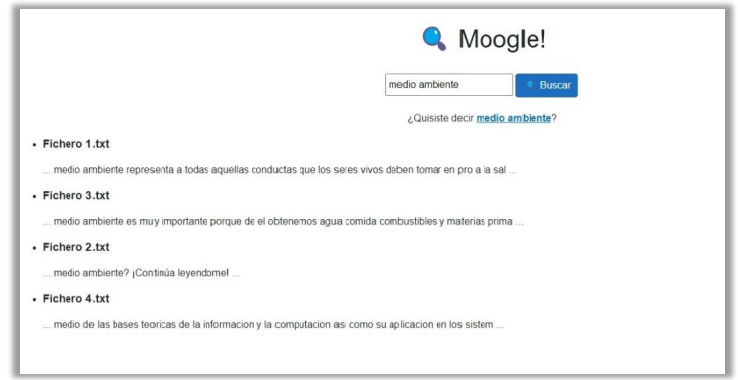
\includegraphics{mooglePaint.png}
	\caption{Funcionamiento Moogle}
\end{figure}
\end{frame}

\end{document}